\documentclass[10pt,a4paper,oneside]{article}

\usepackage{listings}
\usepackage{color}

\definecolor{codegreen}{rgb}{0,0.6,0}
\definecolor{codegray}{rgb}{0.5,0.5,0.5}
\definecolor{codepurple}{rgb}{0.58,0,0.82}
\definecolor{backcolour}{rgb}{0.95,0.95,0.92}
 
\lstdefinestyle{mystyle}{
    backgroundcolor=\color{backcolour},   
    commentstyle=\color{codegreen},
    keywordstyle=\color{magenta},
    numberstyle=\tiny\color{codegray},
    stringstyle=\color{codepurple},
    basicstyle=\footnotesize,
    breakatwhitespace=false,         
    breaklines=true,                 
    captionpos=b,                    
    keepspaces=true,                 
    numbers=left,                    
    numbersep=5pt,                  
    showspaces=false,                
    showstringspaces=false,
    showtabs=false,                  
    tabsize=2
}
 
\lstset{style=mystyle}


\usepackage[utf8]{inputenc}
\usepackage{verbatim}
\usepackage[T1]{fontenc}
\usepackage{amsmath}
\usepackage{amsfonts}
\usepackage{amssymb}
\usepackage{graphicx}
\usepackage[left=2cm,right=2cm,top=2cm,bottom=2cm]{geometry}
\usepackage{multicol}
\usepackage{amsthm}
\author{Baptiste Chanus}

\title{Utilisation d'IA pour anticiper les pannes des architectures en nuage basées sur des micro-service et des conteneurs}

\begin{document}

\begin{center}

\vspace{0.8cm}

\begin{Large}
Utilisation d'IA pour anticiper les pannes des architectures en nuage basées sur des micro-service et des conteneurs
\end{Large}
\end{center}

\vspace{0.8cm}

\begin{figure}[h!]
\centering
\includegraphics[scale=0.5]{./images/PNG/scc-logo.png}
\end{figure}

\vspace{0.8cm}

Author: Chanus Baptiste\\
Coordinator: Aubertin Michael\\
Contact: maubertin@fr.scc.com\\

\vspace{0.8cm}

\begin{abstract}
Dans l’ensemble de l’industrie, de nombreux systèmes reposent sur la stabilité du cloud, du réseau, du datacenter et des composants logiciels. Ainsi, chaque application doit être disponible la plupart du temps. En outre, le modèle de gouvernance informatique incite les équipes informatiques à prendre des engagements forts en matière de responsabilité afin de remédier aux pannes le plus rapidement possible. Ce travail concerne un algorithme d’apprentissage dont le but est de donner un indice sur le moment où une indisponibilité va se produire. En coopération avec les systèmes de surveillance utilisés pour collecter les données sur la disponibilité des applications, comme les logiciels basés sur nagios, l’algorithme vise à traiter les données en rassemblant peu de techniques classiques différentes, telles que l’algorithme génétique de réseau neuronal. Cette méthode est cependant en quelque sorte basée sur des pensées empiriques et vise à deviner un échec avant qu'il ne se produise.
\end{abstract}

\vspace{1.2cm}

\begin{multicols}{2}
\section{Introduction}
Les applications contractées s'exécutent avec un délai maximal d'indisponibilité par jour. Ainsi, lorsqu'un incident se produit, une course contre la montre commence. Le problème doit être diagnostiqué et résolu le plus rapidement possible car il engage l'indicateur qualité qu'est le temps d'indisponibilité. Cet  indicateur de performance clés est un des plus importants KPI d’un accord de niveau de service contracté avec des services informatiques de classe industrielle. Nous essayons ici de trouver une solution qui pourrait aider à anticiper ces problèmes afin que le temps de résolution soit le plus court possible.
\\
Lorsque, en 2017, nous avons essayé de trouver une solution au problème, nous avons décidé d'utiliser les fichiers journaux des systèmes de surveillance basés sur Nagios auxquels nous avions accès. Nous pensions que nous pouvions établir un processus d’apprentissage en utilisant uniquement les données de disponibilité de nagios (décrites dans la partie suivante) pour prévoir toute défaillance de l’application. Toute la solution initiale est expliquée en détail tout au long de la première partie, mais repose sur l'hypothèse selon laquelle les modifications apportées à la structure de l'application sont rares, ce qui était une hypothèse cohérente à cette époque.
\\ 
Cependant, les technologies ont évolué et les applications peuvent avoir de petites modifications dans leur structure régulièrement. Cela rend toute forme d'apprentissage assez difficile, car l'entrainement de l'IA est réalisée avec une structure spécifique de l'application. Ce changement d’architecture est généralement celui attendu d’un nouveau type d’infrastructure, comme par exemple les applications conteneurisées orchestrées. C’est pourquoi, dans une deuxième partie, nous nous concentrerons sur la manière de cibler des hôtes spécifiques, ceux qui ont le plus d’influence sur l’état de l’application, afin de pouvoir appliquer notre méthode d’apprentissage précédente à un sous-ensemble de tous les hôtes de l’application qui ne change pas trop. Enfin, nous essaierons également de regrouper certains hôtes de telle sorte que certains puissent être ajoutés ou supprimés du système d'information tout en étant pris en compte et que l'apprentissage ne soit pas affecté par les changements de structure.
\end{multicols}


\begin{multicols}{2}
\section{Méthode basée sur les disponibilités}
Cette première méthode utilise les données de disponibilité nagios, ce qui signifie que nous n’avons accès, pour chaque hôte et service de l’application, qu’au score d'état de disponibilité compris entre 0 et 3 (0: OK, 1: Avertissement, 2: Critique, 3: Inconnu). Nous allons utiliser les données historiques d'anciens journaux pour entrainer un algorithme d'apprentissage automatique combinant deux techniques d'apprentissage. La première s'appuye sur des réseaux de neurones et ensuite un principe d'algorithme génétique que nous utiliserons ensuite sur les données réelles pour prédire la panne de l'application qui en résultera. éventuellement se produire. Cependant, comme expliqué dans l'introduction, cette méthode pose de sérieux problèmes de rigidité car la formation est faite sur la structure d'une application spécifique. Nous allons discuter de cette limite en tant que conclusion de cette méthode.
\subsection{Modelisation des applications}
La modèlisation d'application choisie est un arbre de dépendances. L'application est la racine de l'arborescence, les nœuds internes sont les hôtes et les feuilles sont les services. À chaque nœud, une relation est associée à ses enfants. Cette porte logique indique si tous sont requis pour la disponibilité de ce nœud ou si certains peuvent être en panne sans rendre ce nœud indisponible. Ces relations ne sont que des relations connues, ce qui signifie qu’elles sont explicites et évidentes lors de la conception de l’application. Nous pouvons avoir des relations qui sont impliquées par l'interaction des nœuds internes qui se produit dans un système de la vie réelle sans que nous en soyons conscients, mais elles ne sont pas évidentes lors du processus de création de l'application. (voir ci-dessous Figure~\ref{exampletree})
\end{multicols}

\vspace{0.8cm}

\begin{figure}
\centering
\includegraphics[scale=0.5]{./images/PNG/abrerelation.png}
\caption{Exemple d'arbre}
\label{exampletree}
\end{figure}

\vspace{0.8cm}

\begin{multicols}{2}
Nous définissons également une image comme étant l’état de l’ensemble de l’application, c’est-à-dire l’état de tous ses composants (hôtes et services) à un moment donné. Ceci est représenté sous la forme d'un tableau contenant 4 lignes, une pour chaque état (0-3) et autant de colonnes que d'hôtes et de services. L'état d'un hôte ou d'un service est donné par un booléen dans le tableau (true dans la ligne correspondant à l'état correspondant et false partout ailleurs), illustré à la figure~\ref{tab}

\end{multicols}

\vspace{0.8cm}

\begin{figure}[!h]
\centering
\includegraphics[scale=0.5]{./images/image.png}
\caption{Matrice d'état}
\label{tab}
\end{figure}

\vspace{0.8cm}


\begin{multicols}{2}
\subsection{Traitement des données}
Nous allons utiliser l'apprentissage automatique supervisé. Par conséquent, nous devons étiqueter les données historiques que nous utiliserons pour former notre réseau de neurones. Le réseau de neurones devra deviner le nombre d'époques restant jusqu'à la prochaine panne. Nous devons donc extraire du journal toutes les époques où l'application était inégalable. Ceci peut être réalisé avec une requête à la base de données dans laquelle sont stockées toutes les dates du début et de la fin d'une panne, puis en modulant les images dont l'époque se situe entre le début et la fin.
  De plus, nous devons associer à chaque image le temps restant avant la prochaine panne. Cela peut être fait facilement en utilisant ce que nous avions calculé auparavant.
\\Nous calculons maintenant une moyenne de toutes les images précédant immédiatement une panne. À ce stade, nous avons fait une hypothèse. Nous avons supposé que suffisamment d'informations avaient été collectées pour alimenter le réseau de neurones et qu'une estimation raisonnablement précise serait stockée dans la comparaison entre une image et la moyenne calculée. Nous allons appeler cette image moyenne la référence.
\\La comparaison entre une image et la référence se fait en utilisant un simple calcul de distance entre coordonnées, c’est-à-dire en notant $a_{i}$ les coordonnées de l’image et $r_{i}$ celles de la référence que nous utilisons, pour un $k\in\mathbb{N}$ donné, la formule suivante:

\vspace{0.8cm}

\begin{Large}
\[ d(a, r) = \sqrt[k]{\sum \mid{a_i - r_i}\mid^{k}} \]
\end{Large}

\vspace{0.8cm}

\subsection{Réseaux de Neurones}
Le premier apprentissage de l'algorithme se fait via des réseaux de neurones. Nous allons former un réseau de neurones pour deviner combien de temps il reste avant la prochaine panne. Un réseau avec une structure donnée est l'ensemble de ses poids et biais qui sont les paramètres que nous allons essayer d'évoluer pendant le processus d'apprentissage. Ils vont être initialisés de manière aléatoire, c'est pourquoi, avant l'entrainement, notre réseau peut être résumé à sa structure. Nous allons donc représenter un réseau par deux listes d'entiers. Une qui spécifiera l’entrée du réseau de neurones et une autre pour ses couches cachées (nous n’avons besoin que d’une sortie: la supposition). La première longueur de la liste est le total des entrées du réseau et chaque entier de cette liste sera utilisé comme $k$ dans la formule de distance, ainsi chaque entrée prendra une valeur différente d'une comparaison différente entre l'image et la référence. La deuxième longueur de la liste est le nombre total de couche cachée et le $i-ème$ entier de la liste est la quantité de neurones dans la couche $i$.

\end{multicols}

\vspace{0.8cm}

\begin{multicols}{2}
Once the network is defined we start the learning phase. We use our labelled data to train the network to guess the time until the next outage with the backpropagation algorithm. This classical algorithm do the computation with the labelled data, evaluate the cost i.e. the error made by the network between the result just obtained and the label associated with the data. Then, this cost is used to modify the weights and biases of the network.
The formula to reevaluate the weights $w^l$ and biases $b^l$ is (for the layer $l$):

\vspace{0.8cm}

\begin{Large}
\[ w^l \leftarrow  w^l-\frac{\eta}{m} \sum_x \delta^{x,l} \,{}^t(a^{x,l-1}) \]
\[ b^l \leftarrow b^l-\frac{\eta}{m} \sum_x \delta^{x,l} \]
\end{Large}

\vspace{0.8cm}


Where $\eta$ is the learning rate, which means a coefficient to control the speed of the changes made upon the weights and biases. $m$ is the number of element used to evaluate the changes that have to be made. $\delta$ is the error and $x$ is a piece of training data.
However several problems appears here. First, when we train the network we are minimizing a function of its inputs which is not convex. So, it has not necessarily only one global minimum, we can, for instance, switch two neurones on the same layer. As a consequence, it could converge only to a local minimum.
The second problem is that we have to determine a good set of hyperparameters i.e. the structure lists of the network, the learning rate and the size of the training data.

\subsection{Evolving hyperparameters}
The solution we proposed is a solution for both problem. It consists in applying the principle of genetic algorithm to our neural networks. After every application outage, we'll evaluate the performance of each network with a fitness function that takes into account the difference between the guess, the reality and its score on an evaluation set of historical data randomly selectionned. So with the distance $x\in\mathbb{R}^{+*}$ and the score $y\in[0, 1]$ we set the function fitness $f$ arbitrarily defined by :

\vspace{0.8cm}

\begin{Large}
\[ f(x, y) = y^{\frac{1}{50}+\frac{1}{1+e^{\frac{1}{1+x}}}} \]
\end{Large}

\vspace{0.8cm}

This function has only been chosen for its shape illustrated on Figure ~\ref{fonction}

\end{multicols}

\vspace{0.8cm}

\begin{figure}[!ht]
\centering
\includegraphics[scale=0.5]{./images/fitness.png}
\caption{Fitness evaluation for several values of y}
\label{fonction}
\end{figure}

\vspace{0.8cm}

\begin{multicols}{2}
At the beginning we create a population of multiple neural networks that we train separatly from different starting parameters (structure, weights and biases). During the analysis we can use the computation of all these networks. Because they started their training from different configurations they propably didn't converge to the same minimum of the function, thus we increase the probability of getting close to a global minimum. 
\\We use all the guesses from all of the networks in the population to get the amount of time we are trying to predict. Then after the application outage we apply the fitness function we introduced above to evaluate individualy the networks (Figure~\ref{pop}) and we generate the next generation using the ones with best results. To perform the selection we normalize all the score so that the total sum is $1$ and we randomly select some networks, the higher their score the higher the probability of being selected.
\end{multicols}

\vspace{0.8cm}

\begin{figure}[!ht]
\centering
\includegraphics[scale=0.5]{./images/PNG/Population.png}
\caption{A population of network}
\label{pop}
\end{figure}

\vspace{0.8cm}

\begin{multicols}{2}
In the process we also add little mutations to the hyperparameters so that we have less chance of getting stuck in a non-optimal configuration. This method also solved the problem of choosing the set of hyperparameters because they are evolving throughout the execution of the algortihm.
With two given network another is created by generating an empty list we fill with elements of a list or the other with probability $\frac{1}{2}$. Then with a little probability called $mutation ~rate$ we introduce mutations which can be either a little variation of an integer in the lists or of the size of each list.

\subsection{Conclusion and limits}
This method can be pretty efficient because we can also collect data from past runs to determine the best structure to start the genetic principle with, which could be seen as another form of learning. However eventhough some part of it could be useful the full method is not feasible because it's unadapted to the new standard architectures of application. Indeed the whole process lies on the training of neural networks that was made using a specific architecture of the application and it shall not evolve during the execution of the algorithm for two big reasons. The first is that the learning would be, in the best case, far less efficient and the second problem is that the comparison is made coordinate by coordinate with an image calculated from historical data. Thus we couldn't compare new images with the old mean and the whole algorithm falls apart.

This indicates a path to follow. We should find a way to identify which variables of the application are the most impactful. This is an interesting question because identifying these variable would not only making possible to restrain the number of data used to feed the neural network, but would allow to add new ones without directly breaking the whole training. Indeed, if the newly introduced variable is important the training could be done later without preventing the comparison. Furthermore, this would be a relevant information to help the diagnosis of an application. This is why the following part will focus on the identification of these variables. With this in mind analazing raw data will be more relevant hence we wont use the monitoring state data but directly values obtained from sensors. Therefore some new method of learning will eventually be explored.

\section{Raw data enhancements}
We need more adaptability because legacy applications weren't changing their achitecture often, they were designed following the Figure~\ref{omodl} schema. This model however didn't allow a lot of optimisations. Therefore now, to adapt to the demand, application are now based on a more horizontal or distributed model as illustrated on Figure~\ref{nmodl}. This cause the infrastructures of the application to change more often. This problem will be discussed in the following part.
\end{multicols}

\begin{figure}[!ht]
\centering
\includegraphics[scale=0.40]{./images/PNG/Application_legacy.png}
\caption{Legacy architecture}
\label{omodl}
\end{figure}

\vspace{0.5cm}

\begin{figure}[!ht]
\centering
\includegraphics[scale=0.60]{./images/PNG/micro_archi.png}
\caption{Cloud and micro architecture}
\label{nmodl}
\end{figure}


\begin{multicols}{2}
We extend here our scope of possibility to all the types of data because we need to solve the rigidity problem of the previous method. First we'll try to find a way of selecting the most influential hosts in the application i.e. the hosts for whom a variation of behavior has an important impact on the whole application. Then, we'll find a way to organize hosts into groups with common behaviors so that we can analyze the mean of the total group. Once done, we'll be able to add and remove hosts from these group without losing the learning. We expect it would also allowed more data to be used during the training of the algorithm.
\end{multicols}

\vspace{0.8cm}

\begin{multicols}{2}

\subsection{Feature selection}
\subsubsection{Signal Processing}
The signal we get from the historical data is full of small variations that may be due to measure errors or changes that are periodical parasite which are irrelevant to treat. Therefore we will try to eliminate as much noise as possible to get a better accuracy in the computation of the influence. Indeed we are going to use a correlation between signals to guess the influence of a variable over another so we have to take into account only the significant event.Furthermore we have to find a proper way of evaluating the influence a node has over another. This overview of our approach is described by Figure~\ref{trng}.
\end{multicols}

\vspace{0.8cm}

\begin{figure}[!ht]
\centering
\includegraphics[scale=0.8]{./images/Apprentissage_V2.png}
\caption{Training phasing}
\label{trng}
\end{figure}

\vspace{0.8cm}

\begin{multicols}{2}
In order to reduce the noise in our signal we'll use some wavelets theory. The choosen method is described in detail in ~\cite{ref1}. Basically we transform the data in wavelet domain with DTCWT - which can be done with the dtcwt library in python for instance (see example code from the documentation below) - we then do the processing, it consists in shrinking the noisy coefficient and finally we recover the de-noised signal by doing the inverse transformation.
\end{multicols}
\begin{lstlisting}[language=Python, caption=Python dtcwt library example]
from matplotlib.pylab import *
import dtcwt


# 1D transform, 5 levels
transform = dtcwt.Transform1d()
vecs_t = transform.forward(vecs, nlevels=5)

# Inverse
vecs_recon = transform.inverse(vecs_t)
\end{lstlisting}


\begin{multicols}{2}
The transformation is a decomposition of the function into a sum of some coefficient multiplied by each vector of a family of wavelets who have specific properties (the theory is explained in detail in the paper). in this work we'll use the Daubechies' wavelets (db11 Figure~\ref{db}) which was chosen using ~\cite{ref2} and referenced papers.
\end{multicols}

\begin{figure}[!h]
\centering
\includegraphics[scale=0.67]{./images/PNG/db11.png}
\caption{Wavelet and scaling function}
\label{db}
\end{figure}

\begin{multicols}{2}
\subsubsection{Influence evaluation}
In this part it is necessary to remember that what we are doing is done before the execution of the application during a learning phase. Therefore, we don't have any constraints in time and the algorithm can be slow.
\\
Our goal is to implement a way to evaluate the influence of each host and service on each other, we can visualize this idea as a graph where the nodes are the hosts and services and the edges are oriented. The edge $(s_i,s_j)$ is linked to the value of the influence $s_j$ has over $s_i$. As on Figure~\ref{graphe}
\end{multicols}


\begin{figure}[!h]
\centering
\includegraphics[scale=0.6]{./images/PNG/Graphe.png}
\caption{Graph example}
\label{graphe}
\end{figure}

\begin{multicols}{2}
The influence is assumed to be in our case the information flow between $s_i$ and $s_j$ so using the Liang-Kleeman information flow ~\cite{ref3} on some data we have, we can compute the value of the edges of the graph.

\subsubsection{Targeting influential hosts}
We now want to sort the nodes by the influence they have in the graph, we'll use the principle of the $page~rank$ algorithm ~\cite{ref4} on the graph where the probability to follow an edge is given by it's value of influence. this is however slightly different than the classical PageRank algorithm because edges have weights. Intuitively it can be seen as a random walk throughout the graph with the probability to follow an edge proportionnal to its weight.

To compute it however, we'll  use the power method witch is a simple and fast way to compute it. Letting $M$ the matrix of transition between the nodes, we obtain it by normalizing the scores of the edges coming out of a node and using them as probability. We compute the rank vector $X$ by starting with an arbitrary $X_0$ and then using :
	\[X_{t+1} = (dM + \frac{1-d}{N}J_N)X_t\]
until we reach :
	\[ \mid{X_t+1 - X_t}\mid < \epsilon\]
where $\epsilon$ is an arbitrarly small parameter, $N$ is the total number of nodes in the graph i.e. the number of hosts and services in the application, $J_N$ is the square matrix of size N containing only ones and finally $d$ is a parameter which represent the probability of stoping the random walk set at $0.85$ because it as been shown by experimentation done by Google that it is the optimal value to have both a decent converging rate and chance of a reaching the $X$ vector we are computing.
\end{multicols}

\begin{lstlisting}[language=Python, caption=Python Power Method]
import numpy as np

def pagerank(M, eps, d=0.85):
    N = M.shape[1]
    X = np.random.rand(N, 1)
    X = X / np.linalg.norm(X, 1)
    X_{t-1} = np.ones((N, 1), dtype=np.float32) * np.inf
    T = (d * M) + (((1 - d) / N) * np.ones((N, N), dtype=np.float32))
    
    while np.linalg.norm(X - X_{t-1}, 2) > eps: 
        X_{t-1} = X
        X = np.matmul(T, X)
    return X

\end{lstlisting}

\begin{figure}[!h]
\centering
\includegraphics[scale=0.5]{./images/PNG/GraphesRandomWalk.png}
\caption{Random walk : initial state}
\label{graphrwb}
\end{figure}

\begin{figure}[!h]
\centering
\includegraphics[scale=0.5]{./images/PNG/GraphesRandomWalk2.png}
\caption{Random walk : advanced state}
\label{graphrw}
\end{figure}

\begin{multicols}{2}
\subsubsection{Conclusion}
Using these different techniques we manage to get a subset of all the hosts and services which are the one with most influence on the whole application. We can focus our learning on these particular variables. Which means that we'll have to deal with architectural changes of the application less often, beside it should also lighten the computations during the training phase. However we'll try to get some more information by grouping the other variables together insuring the flexibility of the application and light computations.\\
\subsection{Grouping features}
Finally when we selected our principal features we cluster all the others in order to be able to adapt to changes in the application architecture. We assumed that the variables that will be removed and added the most often also have limited impact on the global application.\\
We'll use the nearest neighbors process clustering described in this article ~\cite{ref5} (which also expose a K mean algorithm but this one is said to be less effective with small amount of data, which may be the case in our situation) and then we'll use the method described in the first part on the selcted features and a mean of the ones in each cluster.

\end{multicols}

\vspace{0.8cm}

\bibliography{biblio}{}
\bibliographystyle{plain}


\end{document}

